\documentclass[12pt,letterpaper]{article}
\usepackage{graphicx,textcomp}
\usepackage{natbib}
\usepackage{setspace}
\usepackage{fullpage}
\usepackage{color}
\usepackage[reqno]{amsmath}
\usepackage{amsthm}
\usepackage{fancyvrb}
\usepackage{amssymb,enumerate}
\usepackage[all]{xy}
\usepackage{endnotes}
\usepackage{lscape}
\newtheorem{com}{Comment}
\usepackage{float}
\usepackage{hyperref}
\newtheorem{lem} {Lemma}
\newtheorem{prop}{Proposition}
\newtheorem{thm}{Theorem}
\newtheorem{defn}{Definition}
\newtheorem{cor}{Corollary}
\newtheorem{obs}{Observation}
\usepackage[compact]{titlesec}
\usepackage{dcolumn}
\usepackage{tikz}
\usetikzlibrary{arrows}
\usepackage{multirow}
\usepackage{xcolor}
\newcolumntype{.}{D{.}{.}{-1}}
\newcolumntype{d}[1]{D{.}{.}{#1}}
\definecolor{light-gray}{gray}{0.65}
\usepackage{url}
\usepackage{listings}
\usepackage{color}

\definecolor{codegreen}{rgb}{0,0.6,0}
\definecolor{codegray}{rgb}{0.5,0.5,0.5}
\definecolor{codepurple}{rgb}{0.58,0,0.82}
\definecolor{backcolour}{rgb}{0.95,0.95,0.92}

\lstdefinestyle{mystyle}{
	backgroundcolor=\color{backcolour},   
	commentstyle=\color{codegreen},
	keywordstyle=\color{magenta},
	numberstyle=\tiny\color{codegray},
	stringstyle=\color{codepurple},
	basicstyle=\footnotesize,
	breakatwhitespace=false,         
	breaklines=true,                 
	captionpos=b,                    
	keepspaces=true,                 
	numbers=left,                    
	numbersep=5pt,                  
	showspaces=false,                
	showstringspaces=false,
	showtabs=false,                  
	tabsize=2
}
\lstset{style=mystyle}
\newcommand{\Sref}[1]{Section~\ref{#1}}
\newtheorem{hyp}{Hypothesis}

\title{Problem Set 3}
\date{Due: November 19, 2022}
\author{Applied Stats/Quant Methods 1}


\begin{document}
	\maketitle
	\section*{Instructions}
	\begin{itemize}
		\item Please show your work! You may lose points by simply writing in the answer. If the problem requires you to execute commands in \texttt{R}, please include the code you used to get your answers. Please also include the \texttt{.R} file that contains your code. If you are not sure if work needs to be shown for a particular problem, please ask.
	\item Your homework should be submitted electronically on GitHub.
	\item This problem set is due before 23:59 on Sunday November 19, 2023. No late assignments will be accepted.

	\end{itemize}

		\vspace{.25cm}
	
\noindent In this problem set, you will run several regressions and create an add variable plot (see the lecture slides) in \texttt{R} using the \texttt{incumbents\_subset.csv} dataset. Include all of your code.

	\vspace{.5cm}
\section*{Question 1}
\vspace{.25cm}
\noindent We are interested in knowing how the difference in campaign spending between incumbent and challenger affects the incumbent's vote share. 
	\begin{enumerate}
		\item Run a regression where the outcome variable is \texttt{voteshare} and the explanatory variable is \texttt{difflog}.	\vspace{1cm}
        \lstinputlisting[language=R, firstline=1, lastline=25]{PS03_my_answers_daijin_zhou.R}
        \vspace{1cm}
        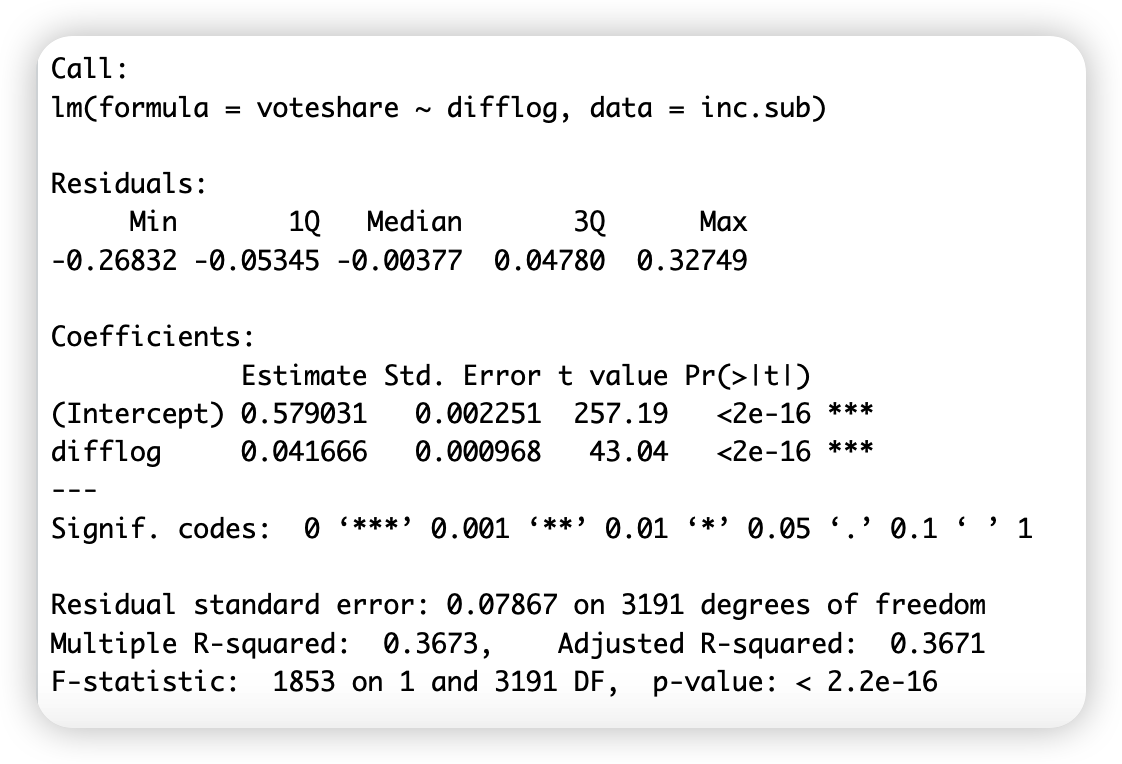
\includegraphics[width=0.99\textwidth]{1-1.png}
        \vspace{1cm}
        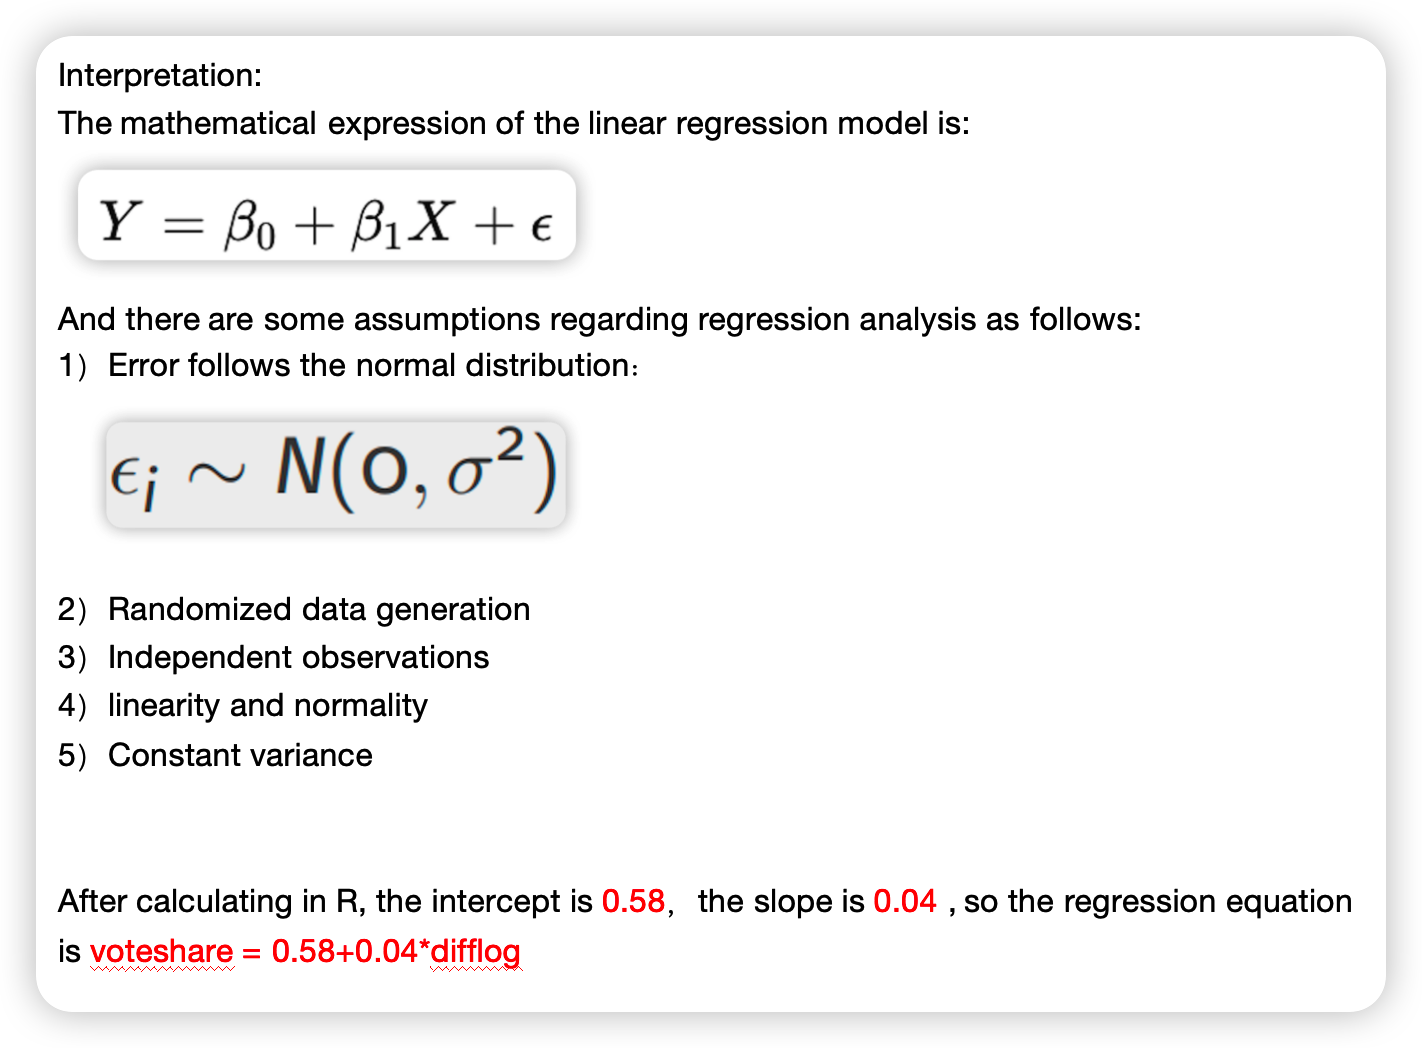
\includegraphics[width=0.99\textwidth]{1-1-inter.png}
		\item Make a scatterplot of the two variables and add the regression line. 	\vspace{1cm}
		\lstinputlisting[language=R, firstline=28, lastline=37]{PS03_my_answers_daijin_zhou.R}
		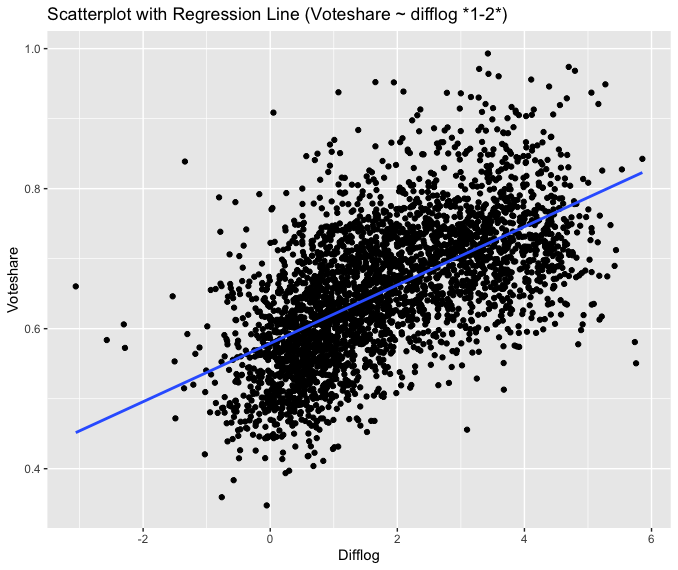
\includegraphics[width=0.99\textwidth]{1-2.png}
		\vspace{1cm}
		\noindent
		Interpretation:\\
		Intercept(0.58) : When difflog = 0 , voteshare = 0.58\\
		Slope(0.04) : because the slope is more than 0, there is a positive relationship between voteshare and difflog; and 1 unit increase in difflog is associated with 0.04 unit increase in voteshare .
		\item Save the residuals of the model in a separate object.	\vspace{1cm}
		\lstinputlisting[language=R, firstline=39, lastline=45]{PS03_my_answers_daijin_zhou.R} \vspace{1cm}
		\item Write the prediction equation.\\
		\noindent
		Interpretation:\\
		Check the validity of this regression equation:\\
		1)Check the significance of coefficients: from the summary of the regression model, the P-values of the coefficients are both less than 0.05 , so the coefficients are significant.\\
		2)Check the residuals are valid in 1-3.\\
		So, The prediction equation is : voteshare-hat = 0.58+0.04*difflog-hat
	\end{enumerate}
	
\newpage

\section*{Question 2}
\noindent We are interested in knowing how the difference between incumbent and challenger's spending and the vote share of the presidential candidate of the incumbent's party are related.	\vspace{.25cm}
	\begin{enumerate}
		\item Run a regression where the outcome variable is \texttt{presvote} and the explanatory variable is \texttt{difflog}.	\vspace{1cm}
		\lstinputlisting[language=R, firstline=65, lastline=82]{PS03_my_answers_daijin_zhou.R}
		\vspace{1cm}
		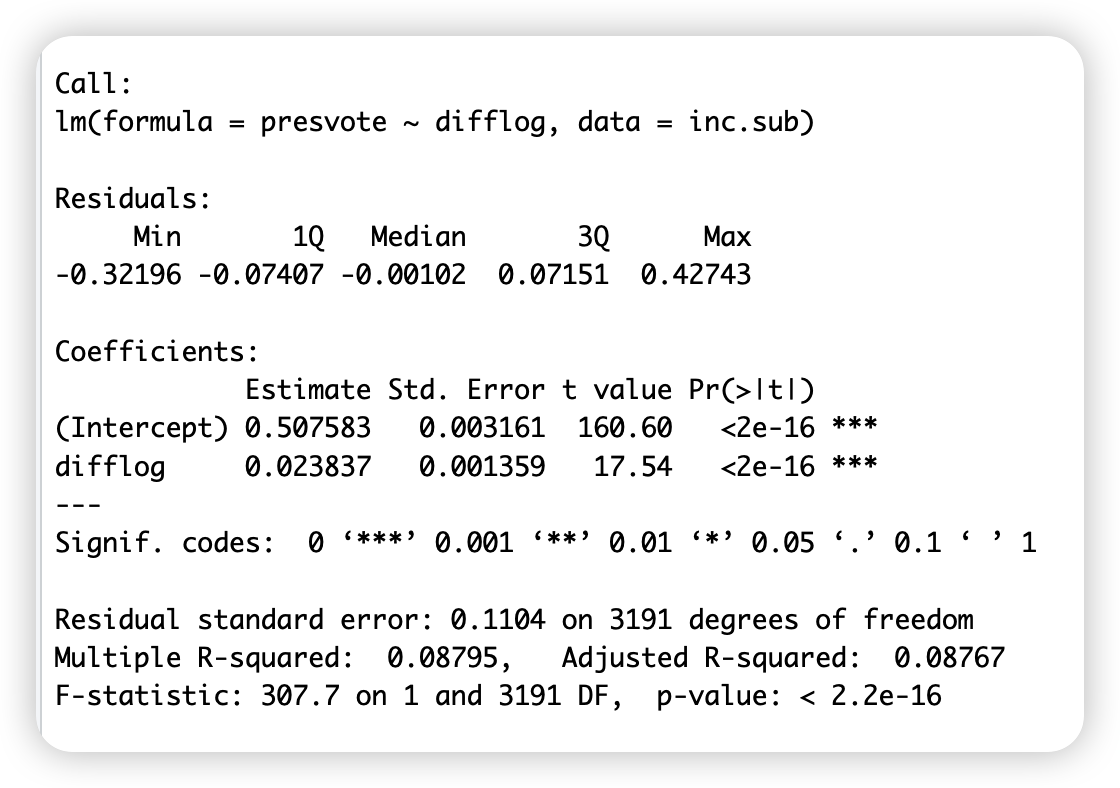
\includegraphics[width=0.99\textwidth]{2-1.png}
		\vspace{1cm}
		\noindent
		Interpretation:\\
		After calculating in R, the intercept is 0.51, the slope is 0.02, so the regression equation is presvote = 0.51+0.02*difflog
		\item Make a scatterplot of the two variables and add the regression line. 	\vspace{1cm}
		\lstinputlisting[language=R, firstline=86, lastline=93]{PS03_my_answers_daijin_zhou.R}
		\vspace{1cm}
		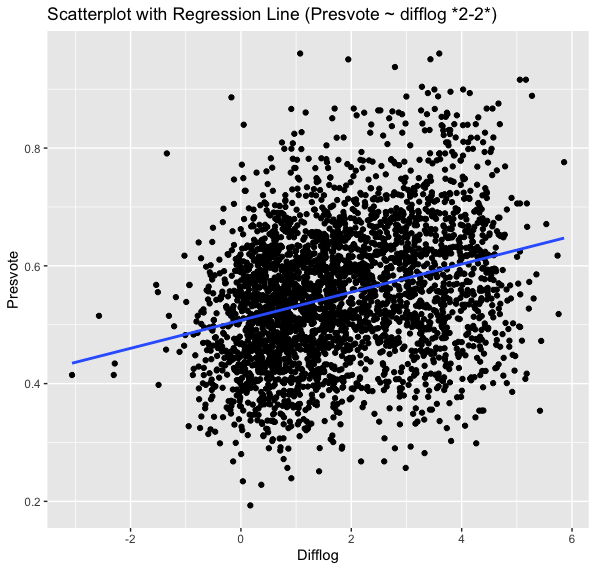
\includegraphics[width=0.99\textwidth]{2-2.png}
		\vspace{1cm}
		\noindent
		Interpretation:\\
		Intercept(0.51): When difflog = 0 , presvote = 0.51\\
		Slope(0.02):  because the slope is more than 0, there is a positive relationship between presvote and difflog; and 1 unit increase in difflog is associated with 0.02 unit increase in presvote .
		\item Save the residuals of the model in a separate object.	\vspace{1cm}
		\lstinputlisting[language=R, firstline=95, lastline=101]{PS03_my_answers_daijin_zhou.R}
		\vspace{1cm}
		\item Write the prediction equation.\\
		\noindent
		Interpretation:\\
		Check the validity of this regression equation:\\
		1)Check the significance of coefficients: from the summary of the regression model, the P-values of the coefficients are both less than 0.05 , so the coefficients are significant.\\
		2)Check the residuals are valid in 2-3.\\
		So, The prediction equation is : presvote-hat = 0.51+0.02*difflog-hat
	\end{enumerate}
	
	\newpage	
\section*{Question 3}

\noindent We are interested in knowing how the vote share of the presidential candidate of the incumbent's party is associated with the incumbent's electoral success.
	\vspace{.25cm}
	\begin{enumerate}
		\item Run a regression where the outcome variable is \texttt{voteshare} and the explanatory variable is \texttt{presvote}.
		\vspace{1cm}			
		\lstinputlisting[language=R, firstline=120, lastline=137]{PS03_my_answers_daijin_zhou.R}
		\vspace{1cm}
		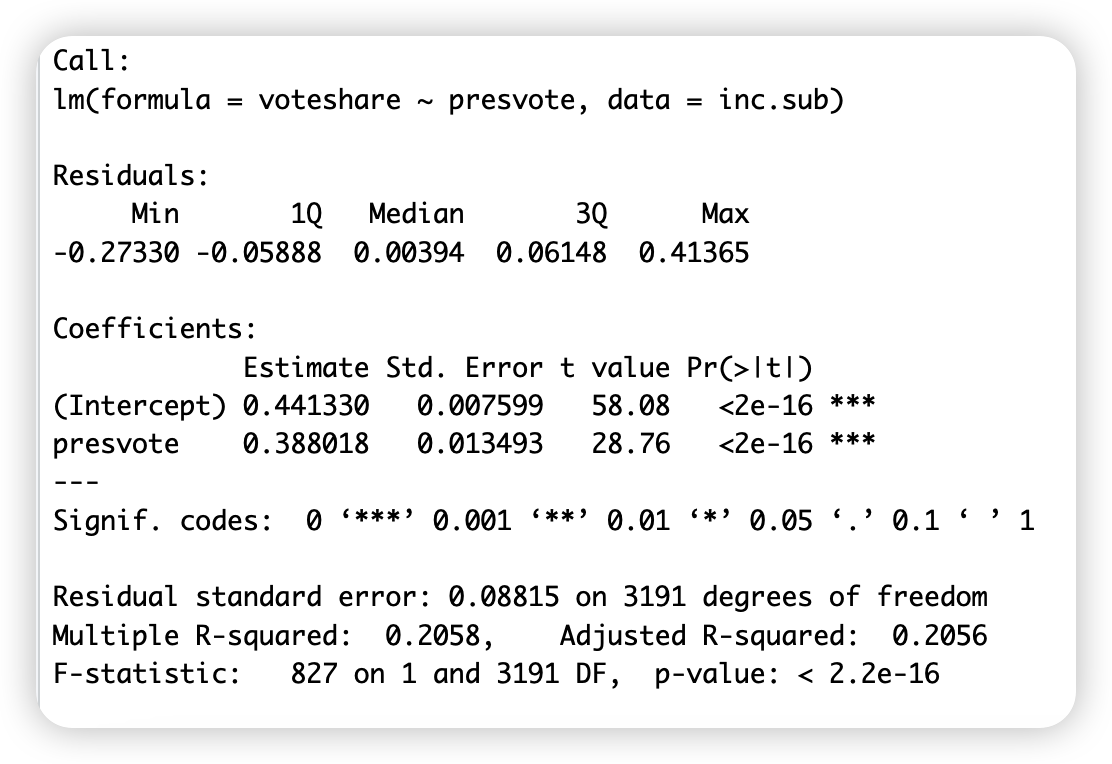
\includegraphics[width=0.99\textwidth]{3_1.png}	
		\vspace{1cm}
		\noindent
		Interpretation:\\
		After calculating in R, the intercept is 0.44,the slope is 0.39, so the regression equation is voteshare = 0.44+0.39*presvote
		\item Make a scatterplot of the two variables and add the regression line. 
		\vspace{1cm}
		\lstinputlisting[language=R, firstline=142, lastline=149]{PS03_my_answers_daijin_zhou.R}
		\vspace{1cm}
		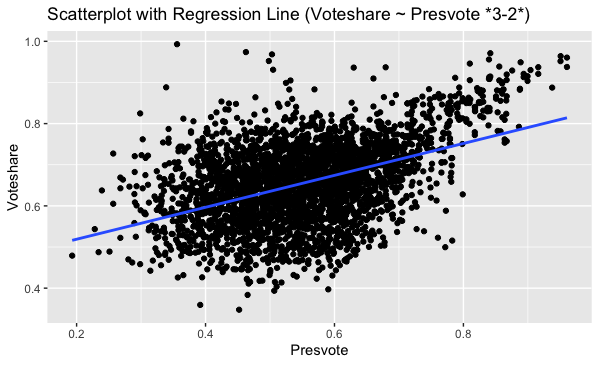
\includegraphics[width=0.99\textwidth]{3_2.png}	
		\noindent
		Interpretation:\\
		Intercept(0.44): When presvote = 0 , voteshare = 0.44\\
		Slope(0.39): because the slope is more than 0, there is a positive relationship between voteshare and presvote; and 1 unit increase in presvote is associated with 0.39 unit increase in voteshare .\\
		\item Write the prediction equation.\\
		\noindent
		Interpretation:\\
		Check the validity of this regression equation:\\
		Check the significance of coefficients: from the summary of the regression model, the P-values of the coefficients are both less than 0.05 , so the coefficients are significant.\\
		So, the prediction equation is : voteshare-hat = 0.44+0.39*presvote-hat
	\end{enumerate}
	

\newpage	
\section*{Question 4}
\noindent The residuals from part (a) tell us how much of the variation in \texttt{voteshare} is $not$ explained by the difference in spending between incumbent and challenger. The residuals in part (b) tell us how much of the variation in \texttt{presvote} is $not$ explained by the difference in spending between incumbent and challenger in the district.
	\begin{enumerate}
		\item Run a regression where the outcome variable is the residuals from Question 1 and the explanatory variable is the residuals from Question 2.	\vspace{1cm}
		\lstinputlisting[language=R, firstline=156, lastline=173]{PS03_my_answers_daijin_zhou.R}
		\vspace{1cm}
		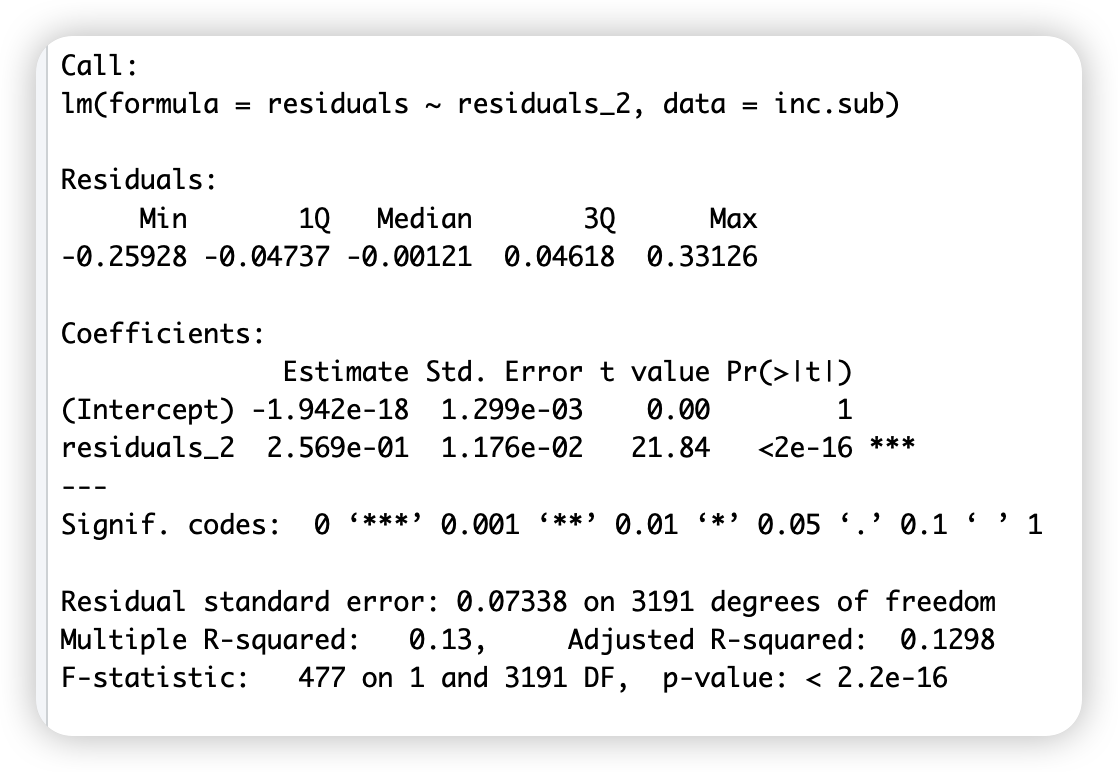
\includegraphics[width=0.99\textwidth]{4-1.png}	
		\vspace{1cm}
		\noindent
		Interpretation:\\
		After calculating in R, the intercept is almost 0, the slope is 0.26, so the regression equation is residuals = 0+0.26*residuals-2
		\item Make a scatterplot of the two residuals and add the regression line. 	\vspace{1cm}
		\lstinputlisting[language=R, firstline=177, lastline=184]{PS03_my_answers_daijin_zhou.R}
		\vspace{1cm}
		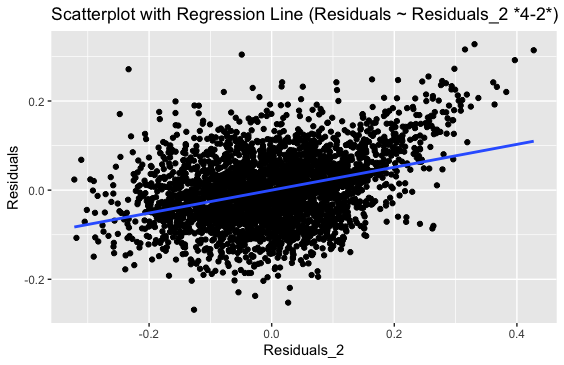
\includegraphics[width=0.99\textwidth]{4_2.png}	
		\vspace{1cm}
		\noindent
		Interpretation:\\
		Intercept(0) : When residuals-2 = 0 , residuals= 0\\
		Slope(0.26) : because the slope is more than 0, there is a positive relationship between residuals and residuals-2; and 1 unit increase in residuals-2 is associated with 0.26 unit increase in residuals .\\
		\item Write the prediction equation.\\
		\vspace{1cm}
		\noindent
		Interpretation:\\
		Check the validity of this regression equation:\\
		Check the significance of coefficients: from the summary of the regression model: the P-value of the intercept is more than 0.05 , so the intercept is not significant, that means the intercept has almost no effect on the model; the P-value of the slope is less than 0.05 , so the slope is significant; \\
		
		So, the prediction equation is : residuals-hat = 0.26*residuals-2-hat
	\end{enumerate}
	
	\newpage	

\section*{Question 5}
\noindent What if the incumbent's vote share is affected by both the president's popularity and the difference in spending between incumbent and challenger? 
	\begin{enumerate}
		\item Run a regression where the outcome variable is the incumbent's \texttt{voteshare} and the explanatory variables are \texttt{difflog} and \texttt{presvote}.	\vspace{1cm}
		\lstinputlisting[language=R, firstline=189, lastline=209]{PS03_my_answers_daijin_zhou.R}
		\vspace{1cm}
		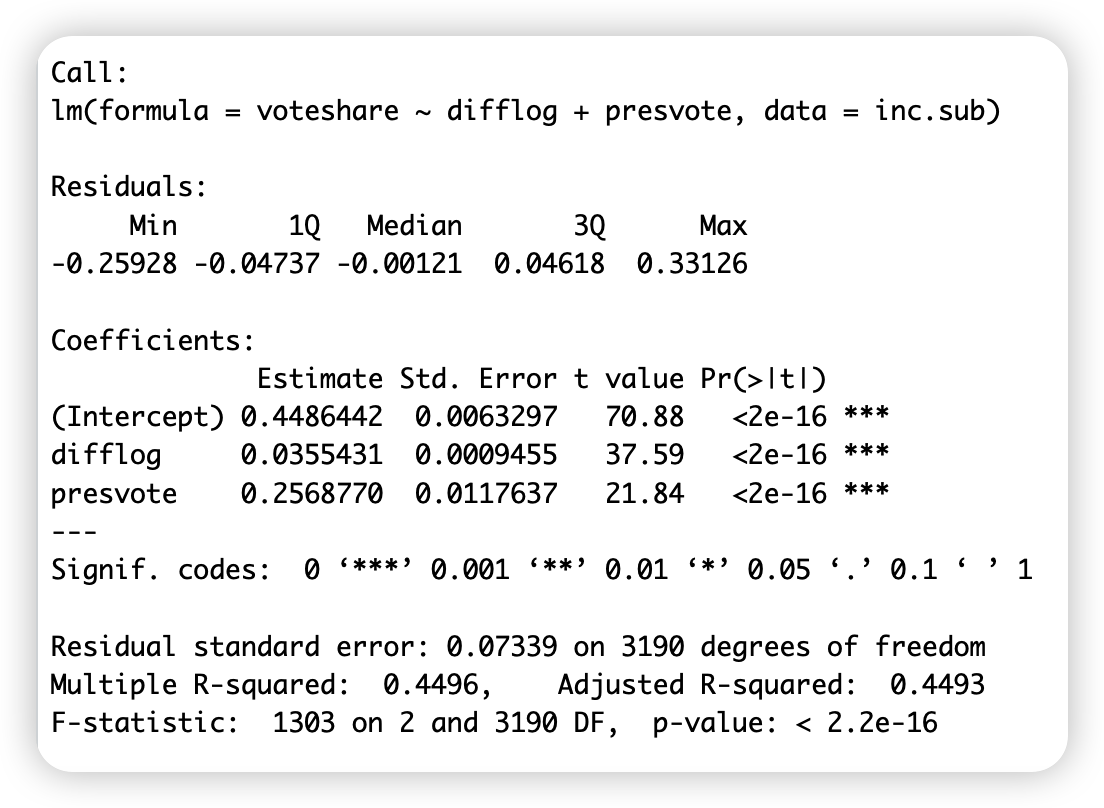
\includegraphics[width=0.99\textwidth]{5-1.png}	
		\vspace{1cm}
		\noindent
		Interpretation:\\
		After calculating in R, the intercept is 0.45, the slope of difflog is 0.04 , and the slope of presvote is 0.26, so the regression equation is voteshare = 0.45+0.04*difflog + 0.26*presvote \\
		
		- Intercept(0.45) : When difflog = 0 and presvote = 0, voteshare = 0.45\\
		- Slope(0.04) : because the slope is more than 0, there is a positive relationship between voteshare and difflog; and with the value of presvote remianing constant, the 1 unit increase in difflog is associated with 0.04 unit increase in voteshare .  \\
		- Slope(0.26) : because the slope is more than 0, there is a positive relationship between voteshare and presvote ; and with the value of difflog remianing constant, 1 unit increase in presvote is associated with 0.26 unit increase in voteshare . \\
		\item Write the prediction equation.\\	\vspace{5cm}
		\noindent
		Interpretation:\\
		Check the validity of this regression equation:\\
		Check the significance of coefficients: from the summary of the regression model, the P-values of the coefficients are both less than 0.05 , so the coefficients are significant.\\
		
		So, the prediction equation is : voteshare-hat = 0.45+0.04*difflog-hat + 0.26*presvote-hat 
		\item What is it in this output that is identical to the output in Question 4? Why do you think this is the case?\\ \vspace{1cm}
		\noindent
		Interpretation:\\
		Comparing the residuals of regression model in Q4 and Q5, they are identical, because there is a certain degree of collinearity between difflog and presvote.
	\end{enumerate}




\end{document}
